\newpage
\section{Cliente}

\subsection{Gestione profilo}

Una volta effettuato con successo il login, è possibile accedere al proprio profilo utente. La schermata principale relativa al profilo apparirà come nella figura sottostante.

\label{Profilo utente}
\begin{figure}[H]
	\centering
	\fbox{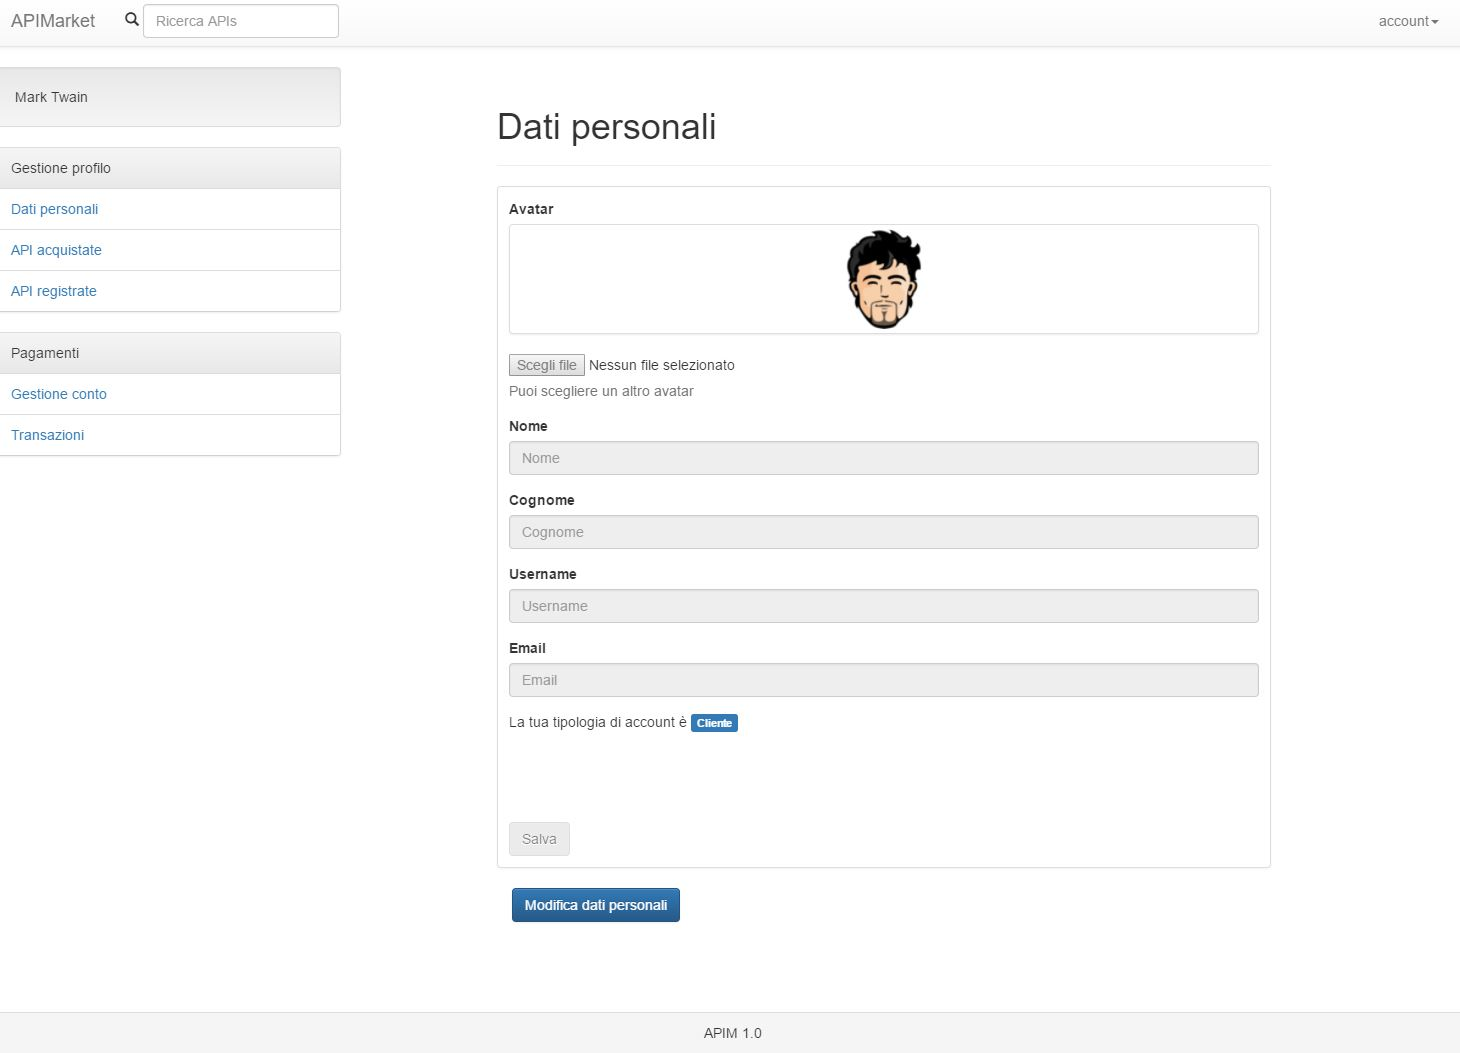
\includegraphics[scale=0.31]{img/APIM_account.JPG}}
	\caption{Profilo utente}
\end{figure}

Dalla schermata si potranno modificare i dati personali, inseriti al momento della registrazione, quali la propria anagrafica o dati relativi all'account quali l'immagine personale. E' visualizzato inoltre a quale gruppo di utenza si appartiene: l'utente registrato semplice infatti è un utente denominato "cliente", mentre l'utente abilitato al caricamento e alla vendita di servizi è denominato utente "Developer".

Tramite il menù laterale è possibile navigare nelle schermate del proprio profilo. Cliccando sulla voce API acquistate si potrà consultare l'elenco delle api attualmente in possesso o acquistate in passato con i relativi dati. 

\subsubsection{API Aquistate}
\label{API acquistate}
\begin{figure}[H]
	\centering
	\fbox{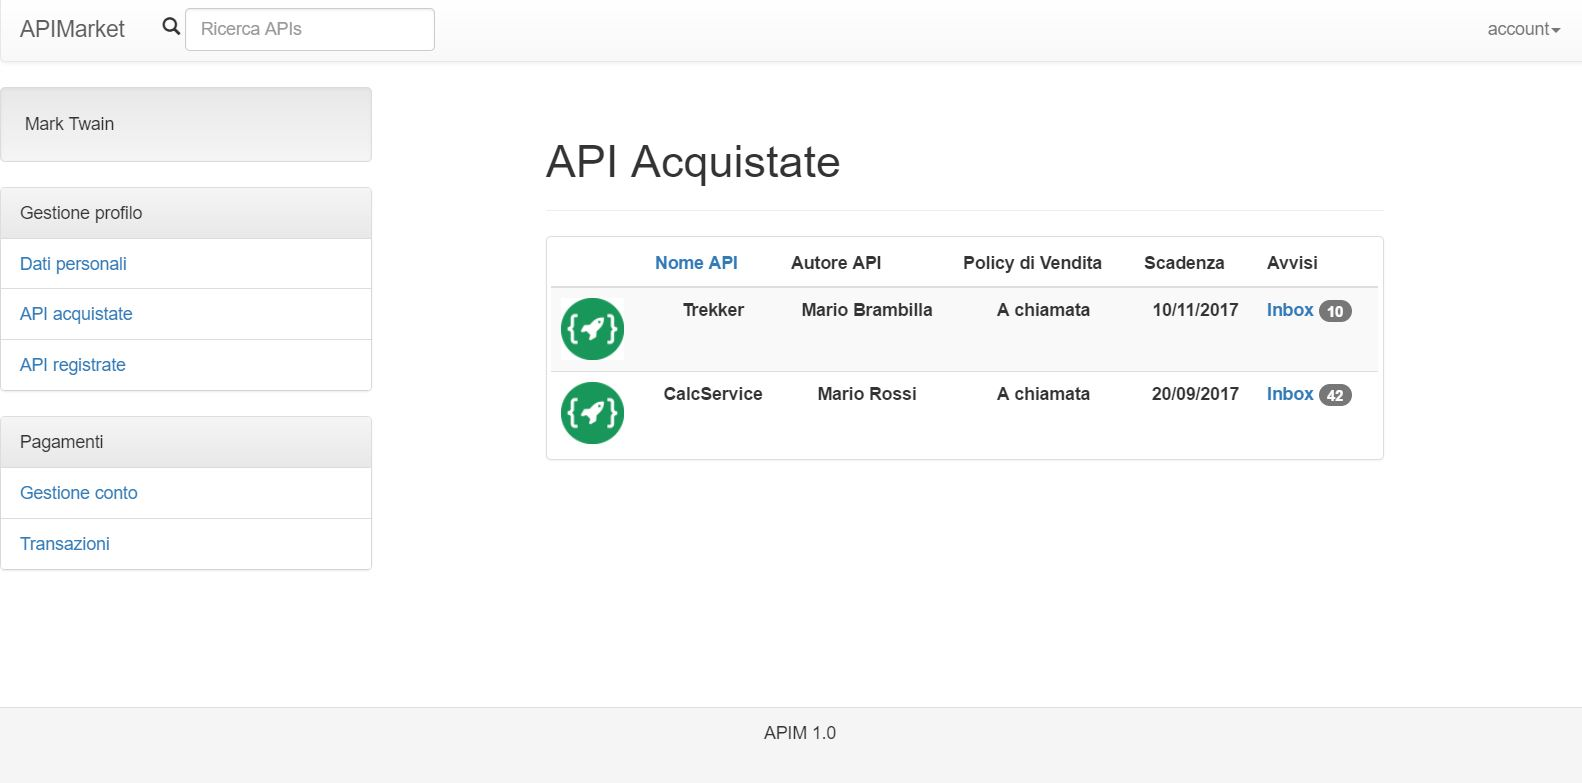
\includegraphics[scale=0.31]{img/APIM_apiAcquistate.JPG}}
	\caption{API acquistate}
\end{figure}
Nell'elenco delle API Acquistate è possibile rinnovare un'API prossima alla scadenza tramite l'apposito pulsante. L'utente effettuerà così una nuova transazione.
\subsubsection{API-Key smarrita}
Tramite la sezione API Aquistate è possibile richiedere una nuova API Key in caso di smarrimento della precendente. cliccando su Nuova chiave API, apparirà un pop-up contenente la nuova chiave, come mostrato nella figura seguente.

\label{Nuova API}
\begin{figure}[H]
	\centering
	\fbox{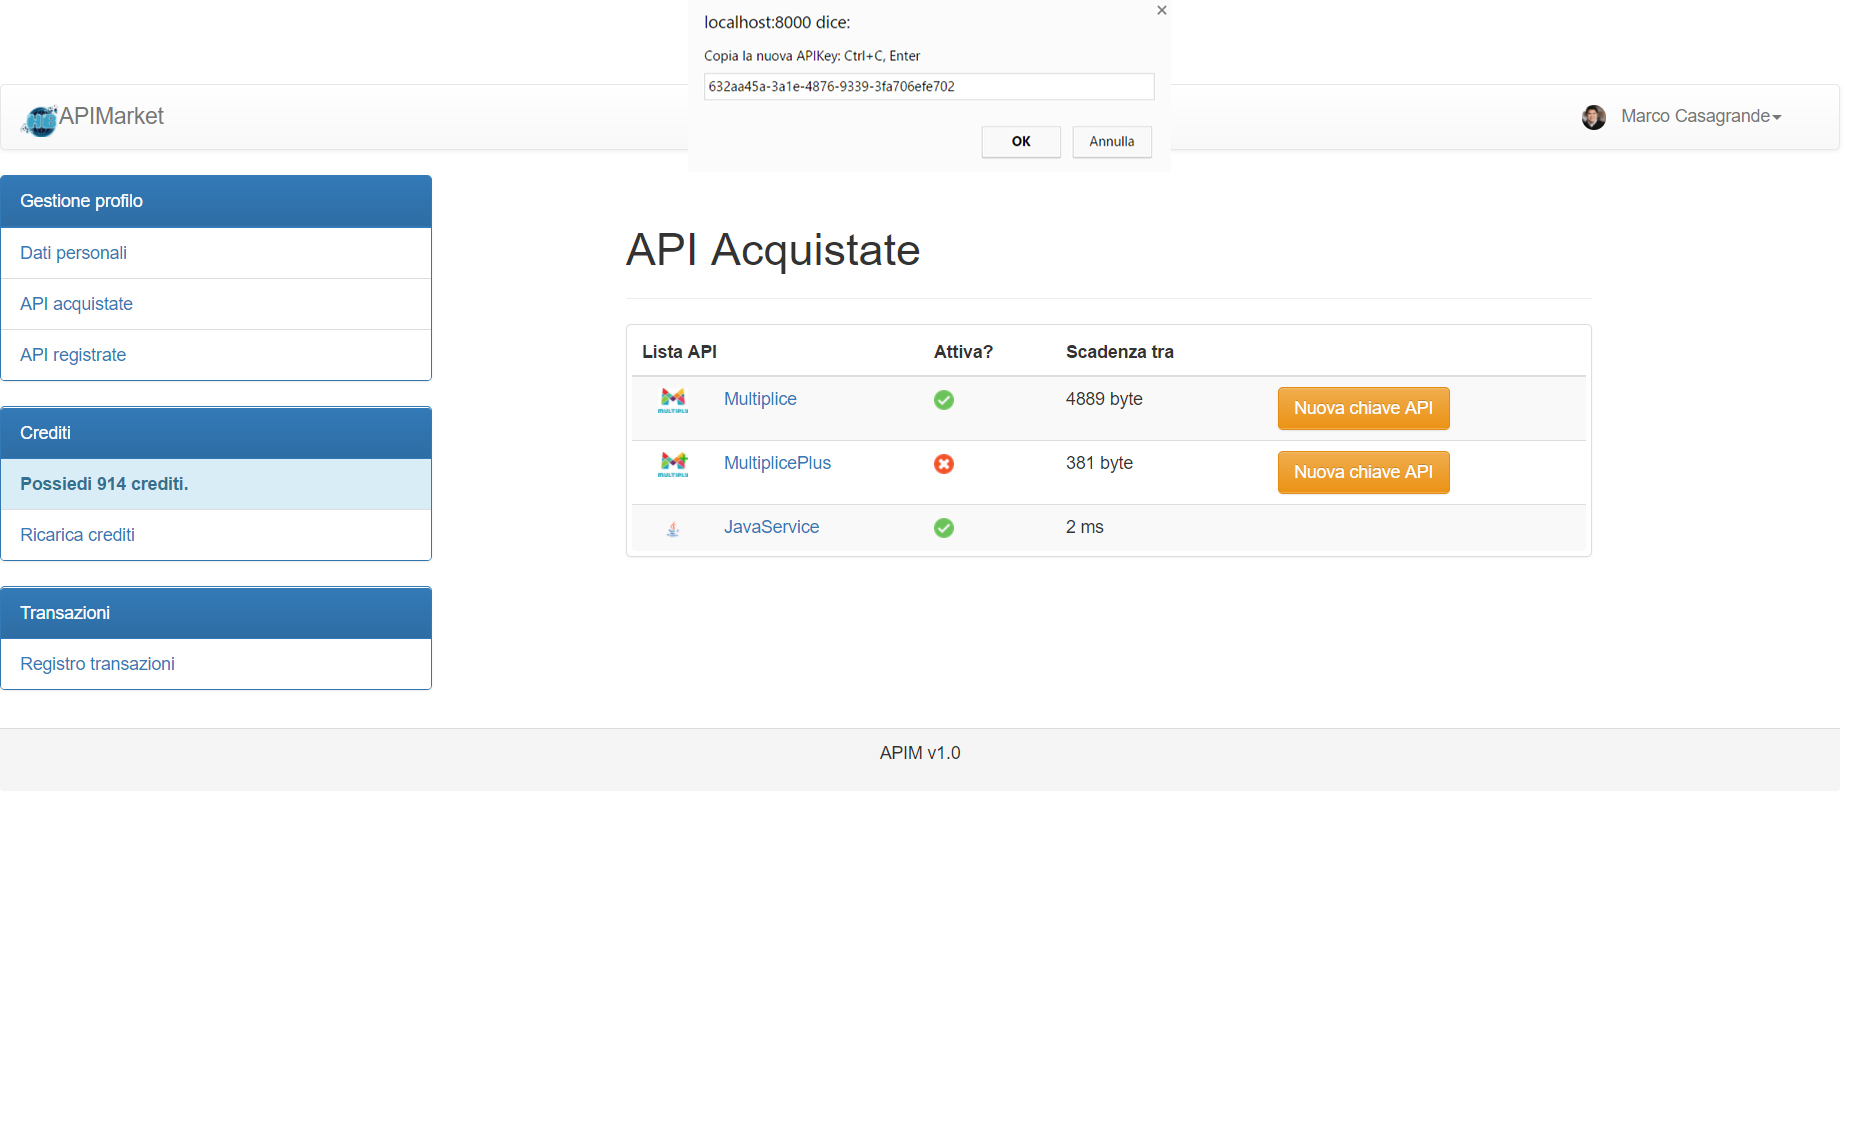
\includegraphics[scale=0.25]{img/APIM_nuovaKey.jpg}}
	\caption{Nuova API}
\end{figure}

\subsubsection{Registro Transazioni}
Ogni cliente può consultare lo storico transazioni dalla propria area personale tramite il menù a sinistra, cliccando su "Registro transazioni". \MakeUppercase{è} possibile visualizzare le ultime dieci, venti o tutte le transazioni tramite un menù a tendina.

\label{Registro Transazioni }
\begin{figure}[H]
	\centering
	\fbox{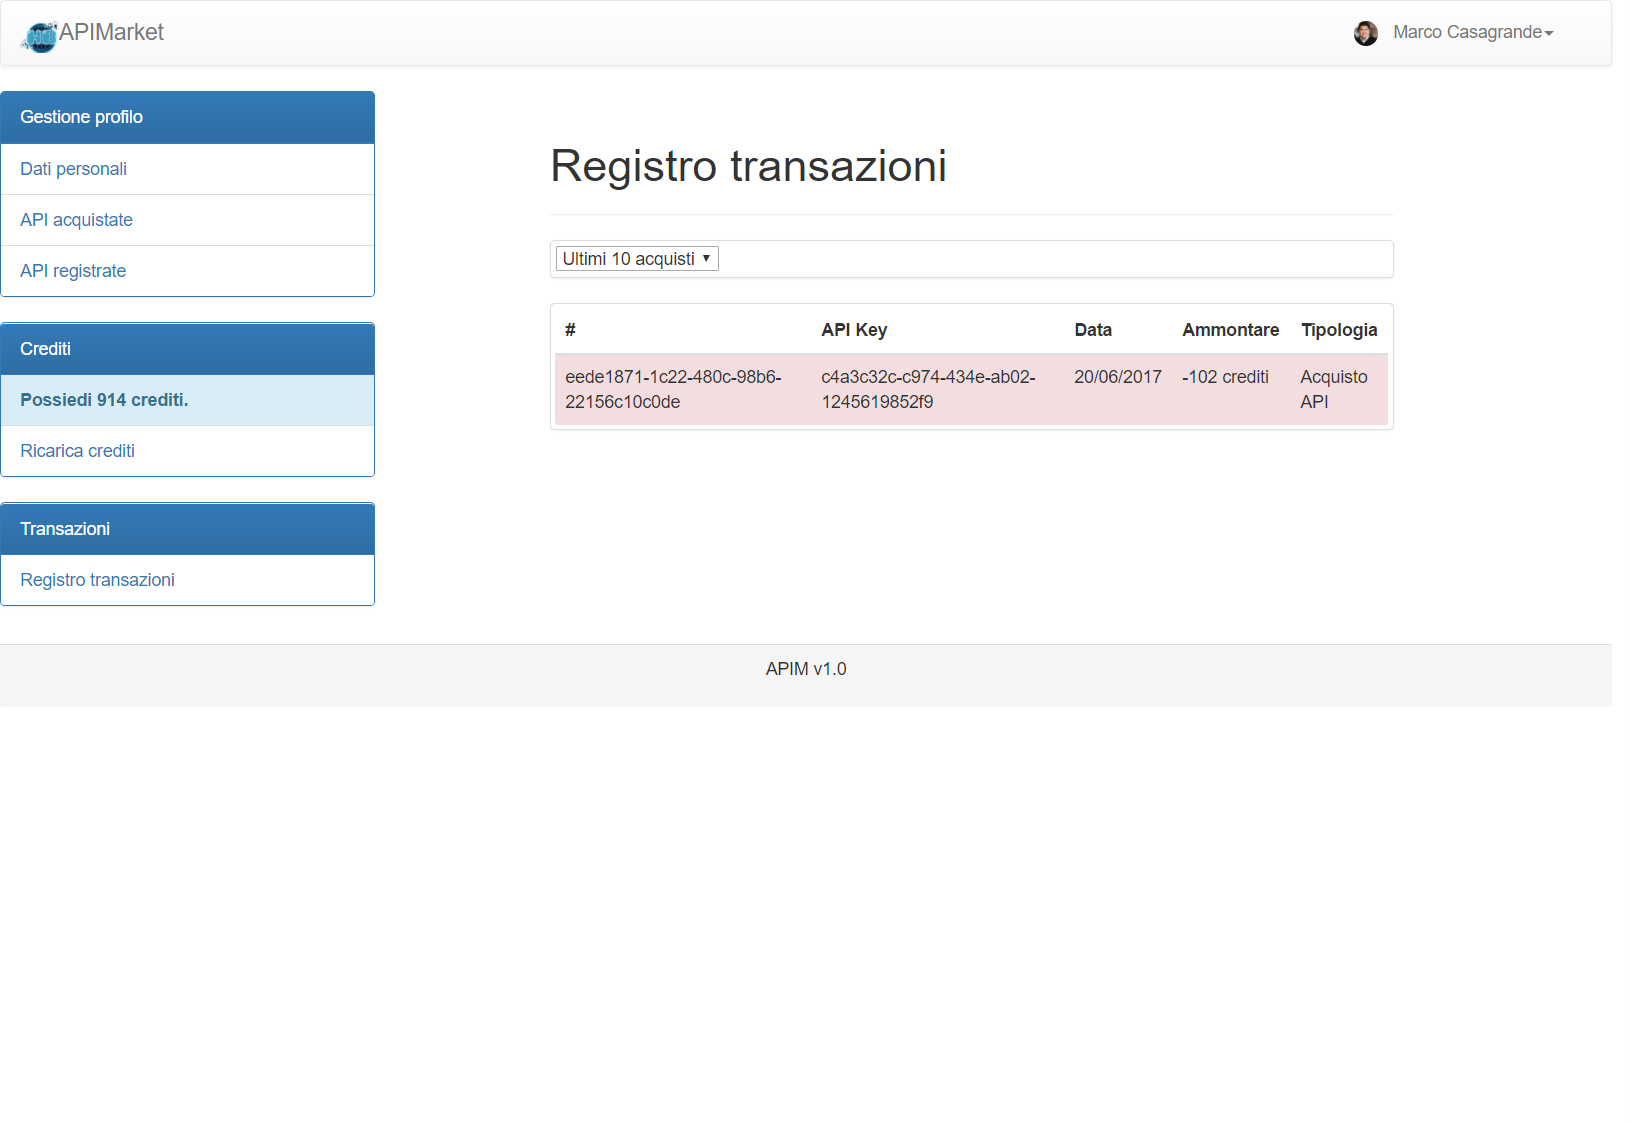
\includegraphics[scale=0.25]{img/APIM_RegistroTransazioni.png}}
	\caption{Registro Transazioni}
\end{figure}

\subsection{Acquisto API}
Un cliente può acquistare una API direttamente dalla pagina di dettaglio API tramite il pulsante Acquista. 

All'interno della pagina il cliente potrà scegliere l'importo da acquistare a seconda della policy dell'API che intende acquistare.  

Una volta completata la transazione, il saldo di crediti sarà aggiornato e l'utente riceverà un API key con la quale potrà utilizzare il servizio acquistato. 

\label{Acquisto API}
\begin{figure}[H]
	\centering
	\fbox{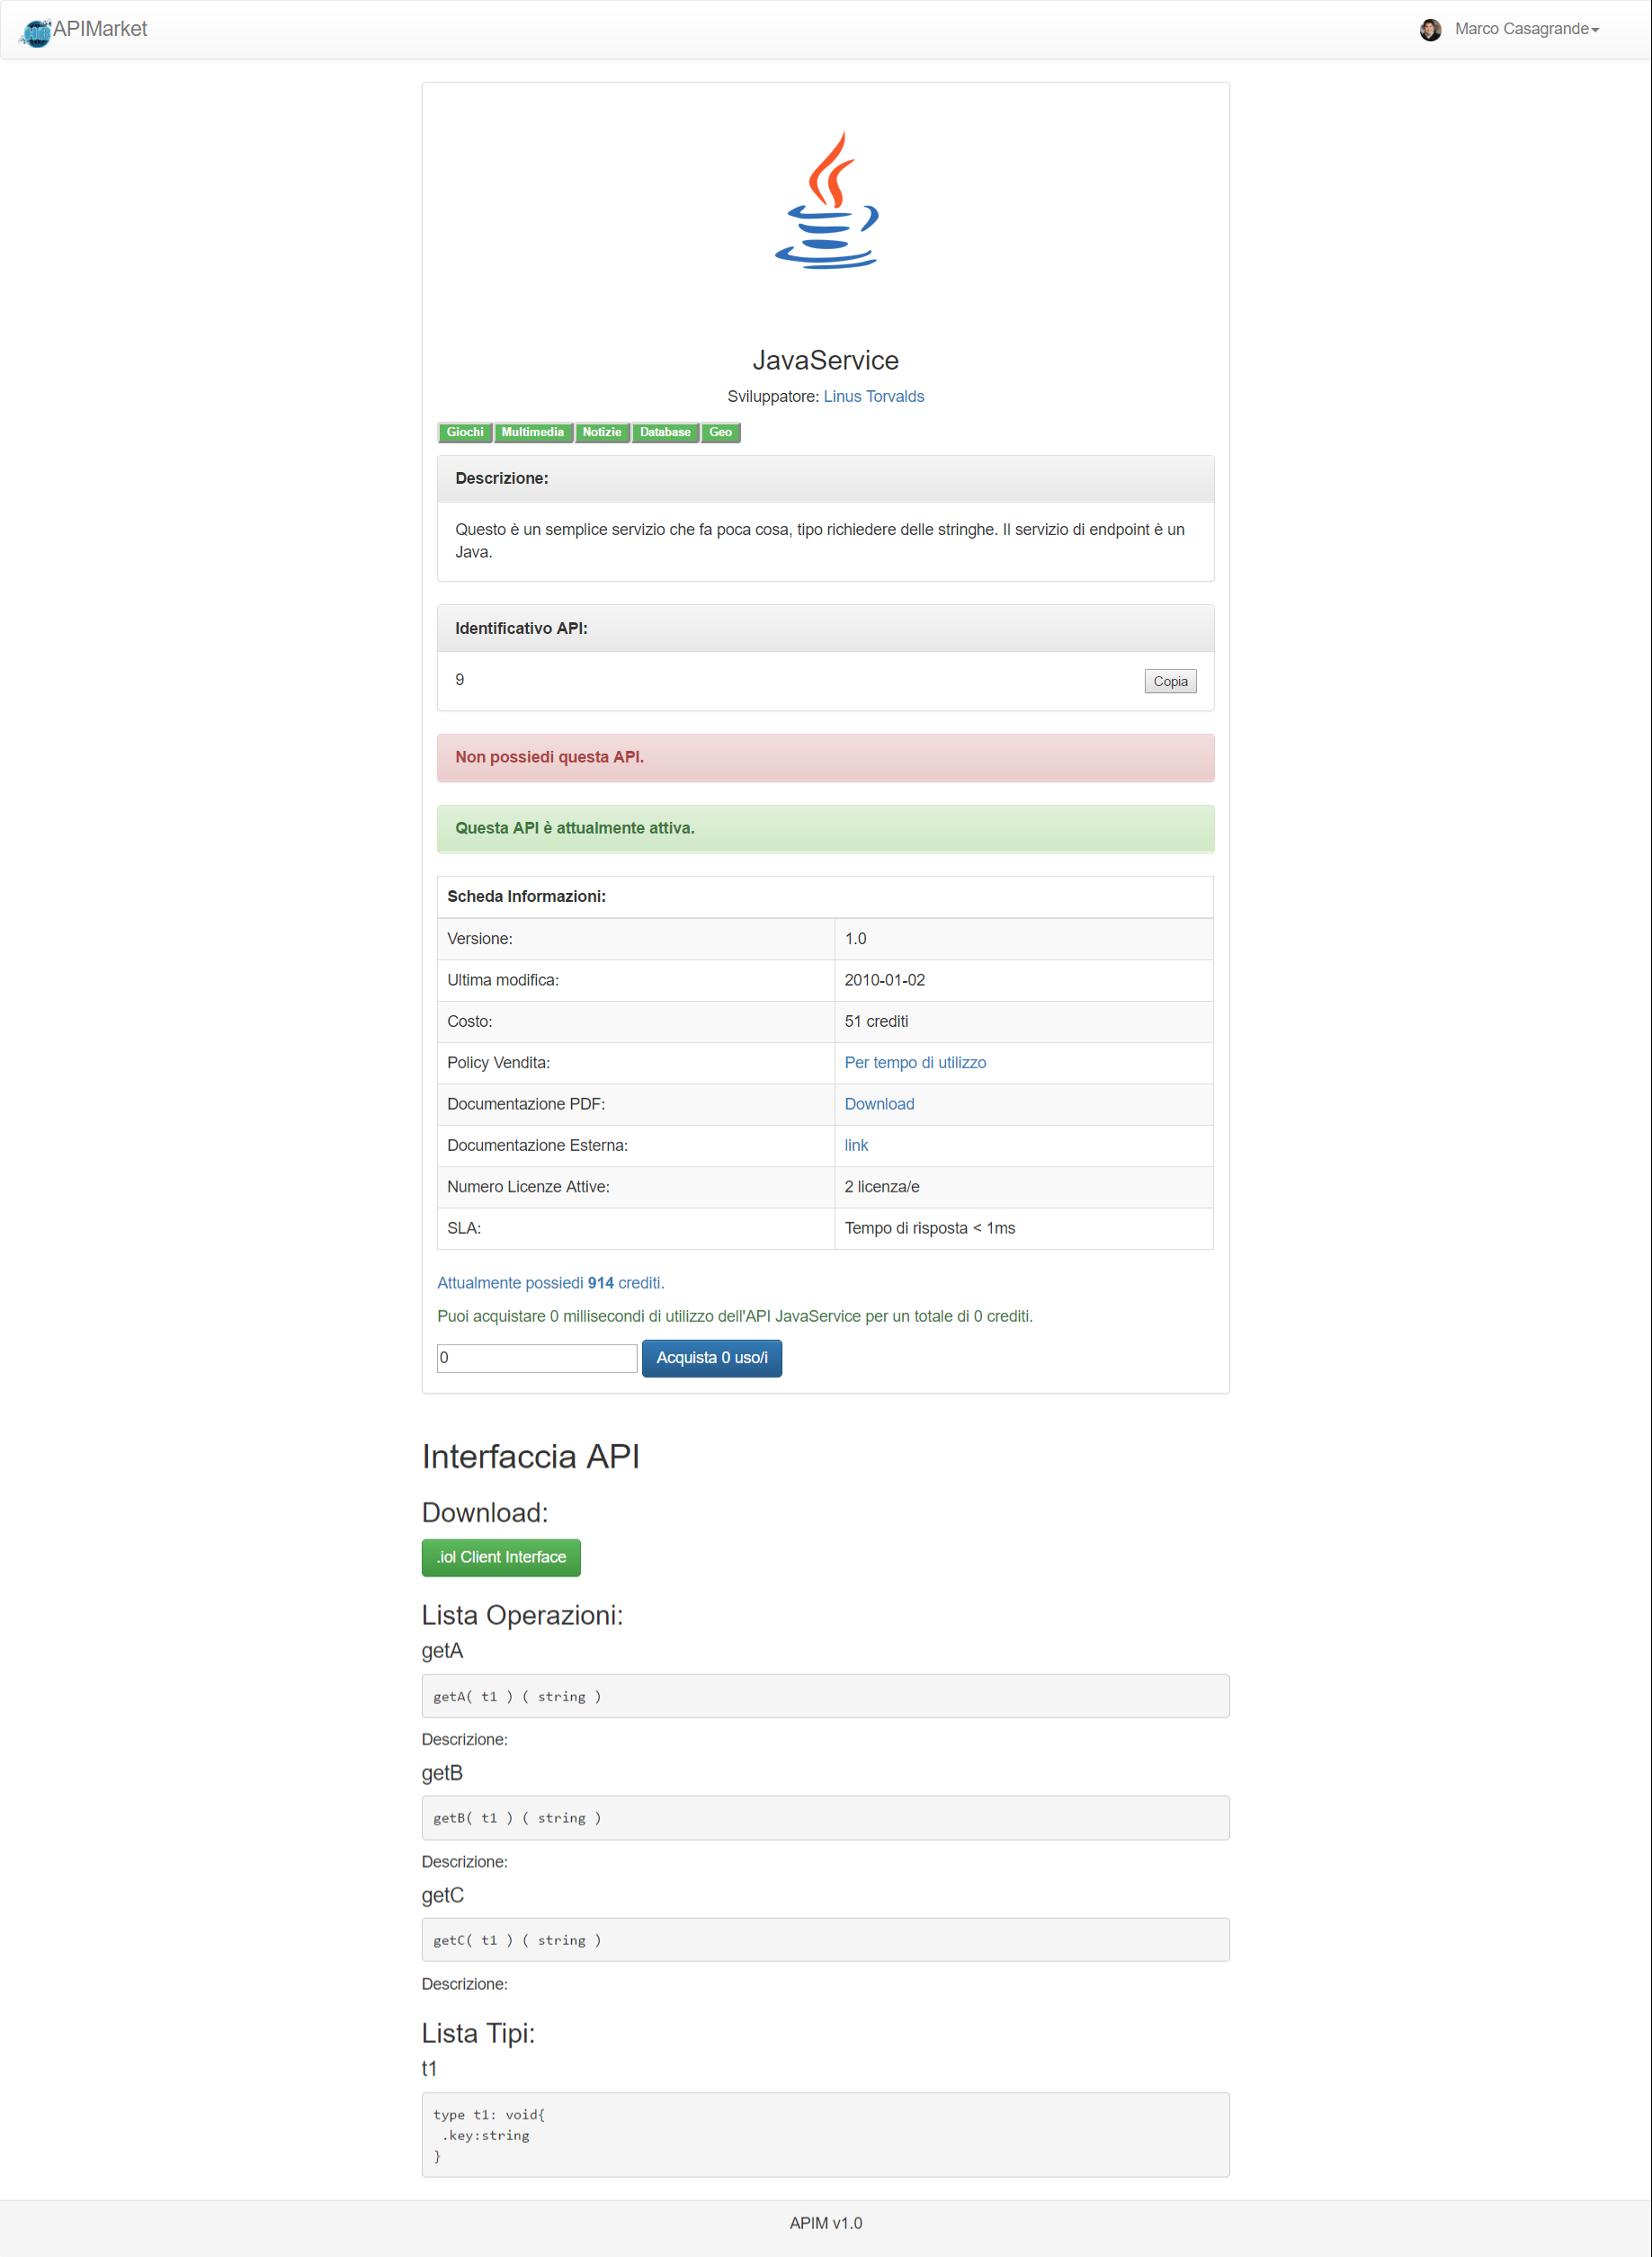
\includegraphics[scale=0.26]{img/APIM_dettaglioAquisto.png}}
	\caption{Acquisto API}
\end{figure}
Una volta concluso l'acquisto dell'API, il cliente attraverso l'interfaccia scaricabile sulla pagina dell'API acquistata e la documentazione inserita dallo sviluppatore, sarà in grado di utilizzare il servizio acquistato.

\subsection{Acquisto crediti}
Dalla gestione del profilo, un utente è in grado di acquistare crediti utilizzabili per pagare le API. Un utente può acquistare un numero di crediti a scelta tra i tagli presenti nell'apposita pagina. 
\label{Acquisto Crediti}
\begin{figure}[H]
	\centering
	\fbox{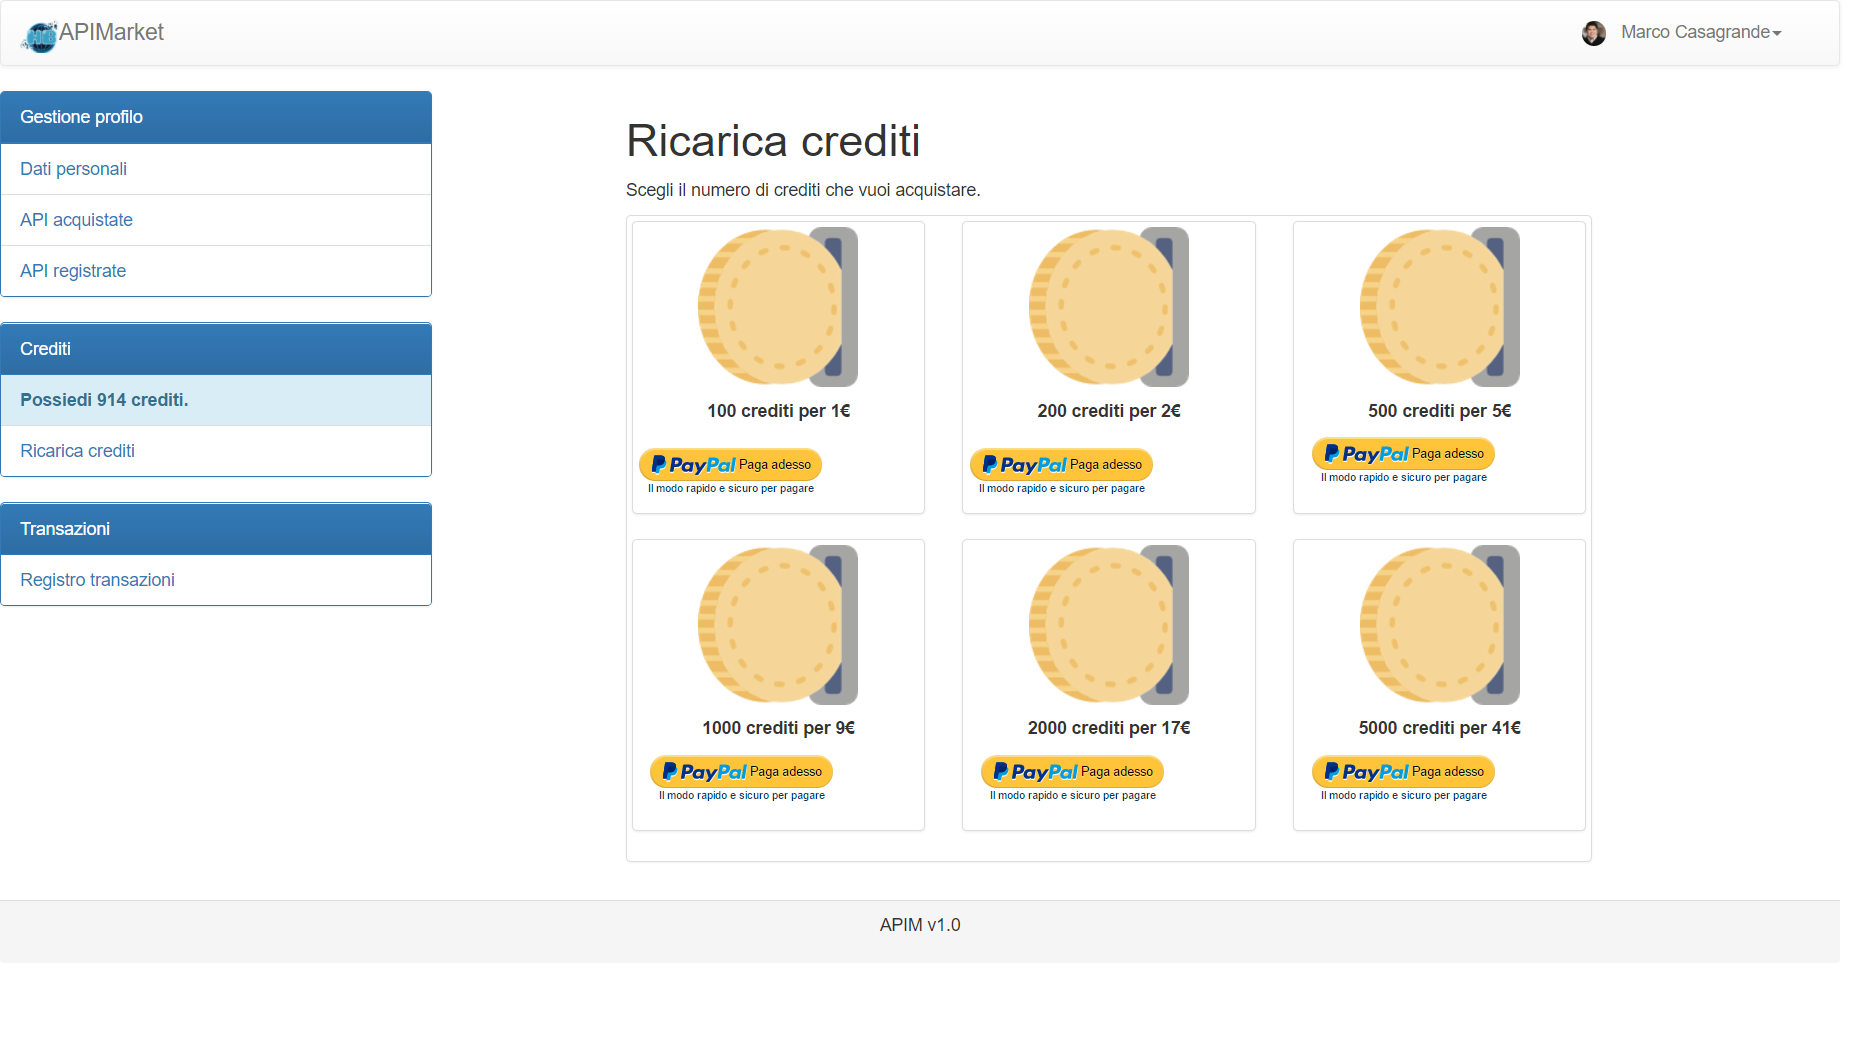
\includegraphics[scale=0.25]{img/APIM_acquistoCrediti.JPG}}
	\caption{Acquisto Crediti}
\end{figure}

Nella pagina successiva l'utente completa la transazione sul sito Paypal e il saldo crediti del suo conto viene aggiornato con i nuovi crediti sommati ai precedenti.

\label{Acquisto Crediti Paypal}
\begin{figure}[H]
	\centering
	\fbox{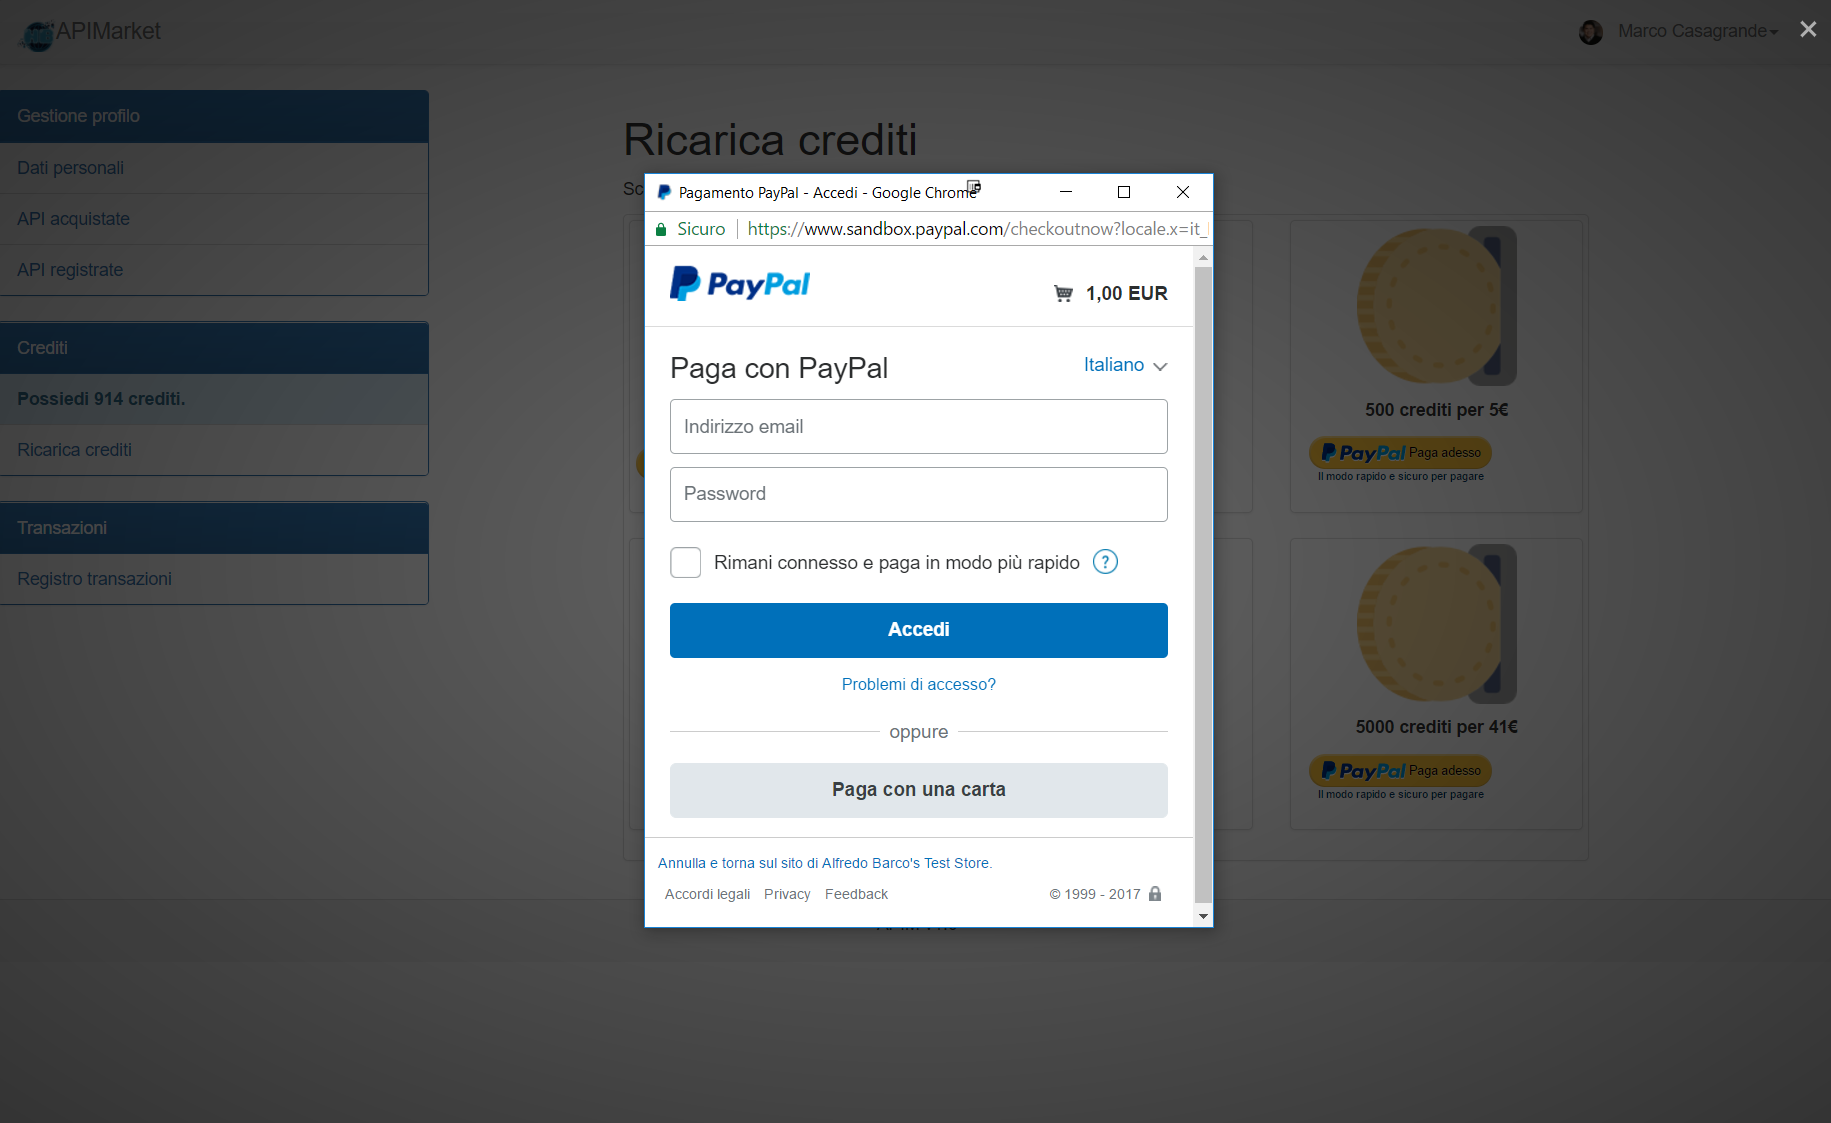
\includegraphics[scale=0.42]{img/APIM_acquistoPaypal.png}}
	\caption{Acquisto Crediti Paypal}
\end{figure}

\subsection{Cambio password}
Dalla gestione del profilo è possibile cambiare la passowrd, inserendo la password attuale e due volte la nuova password. 
\label{Cambio password}
\begin{figure}[H]
	\centering
	\fbox{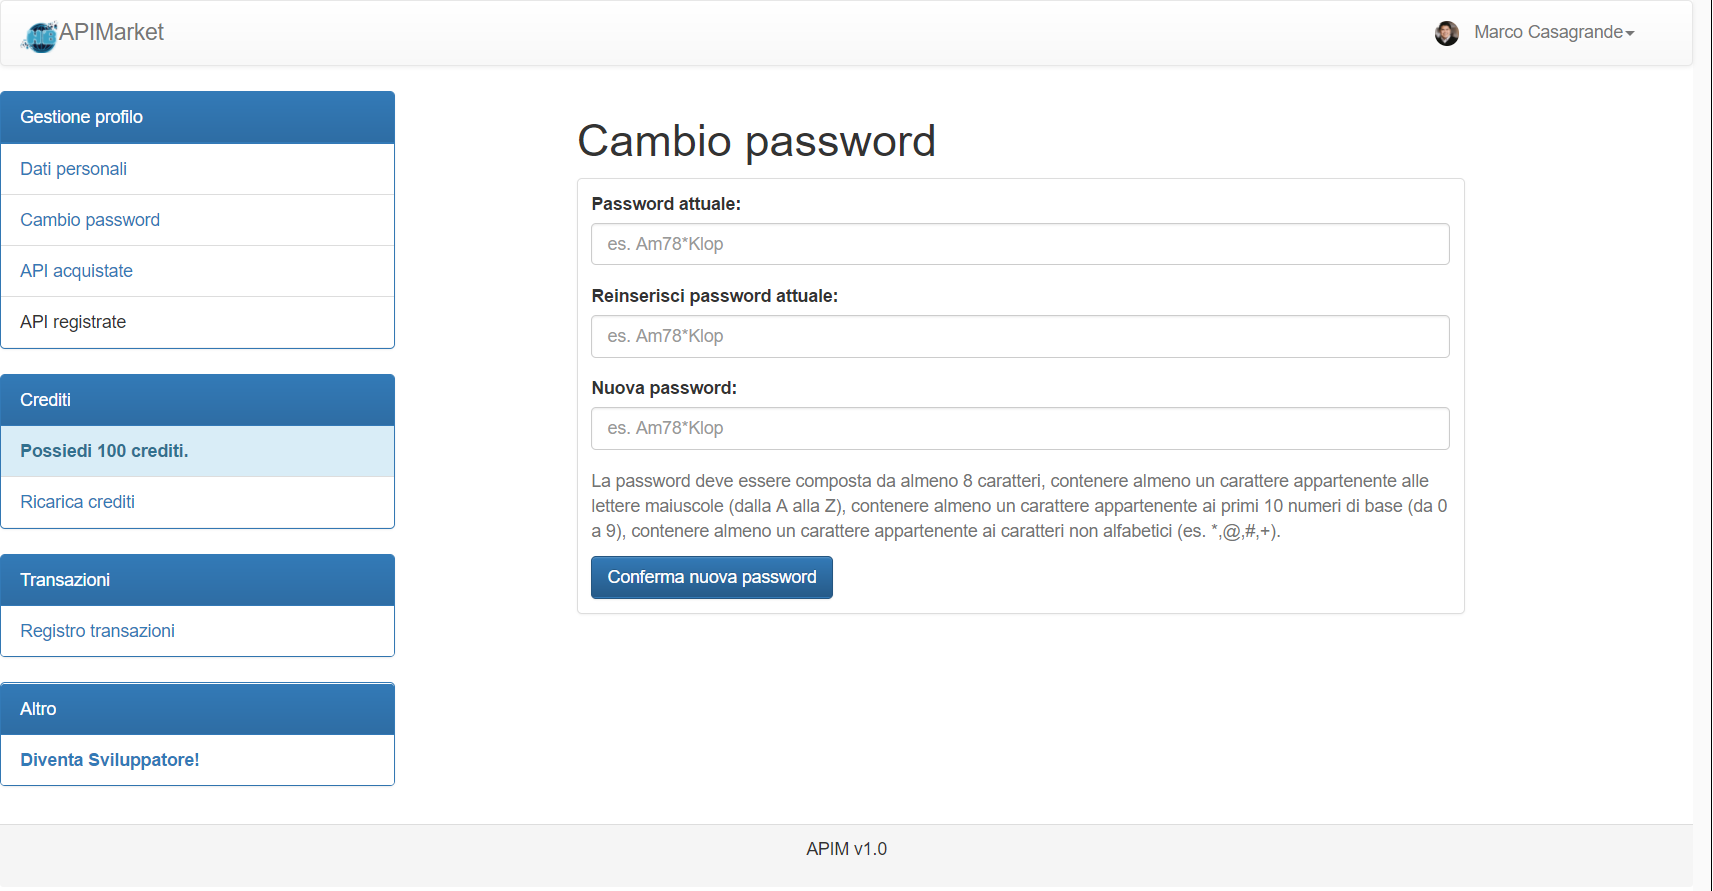
\includegraphics[scale=0.25]{img/APIM_cambioPSW.png}}
	\caption{Cambio password}
\end{figure}
In caso di inserimento di password attuale errata e/o nuova password non conforme allo standard, verrà visualizzato l'errore relativo, come mostrato nella seguente immagine.

\label{Errori cambio password}
\begin{figure}[H]
	\centering
	\fbox{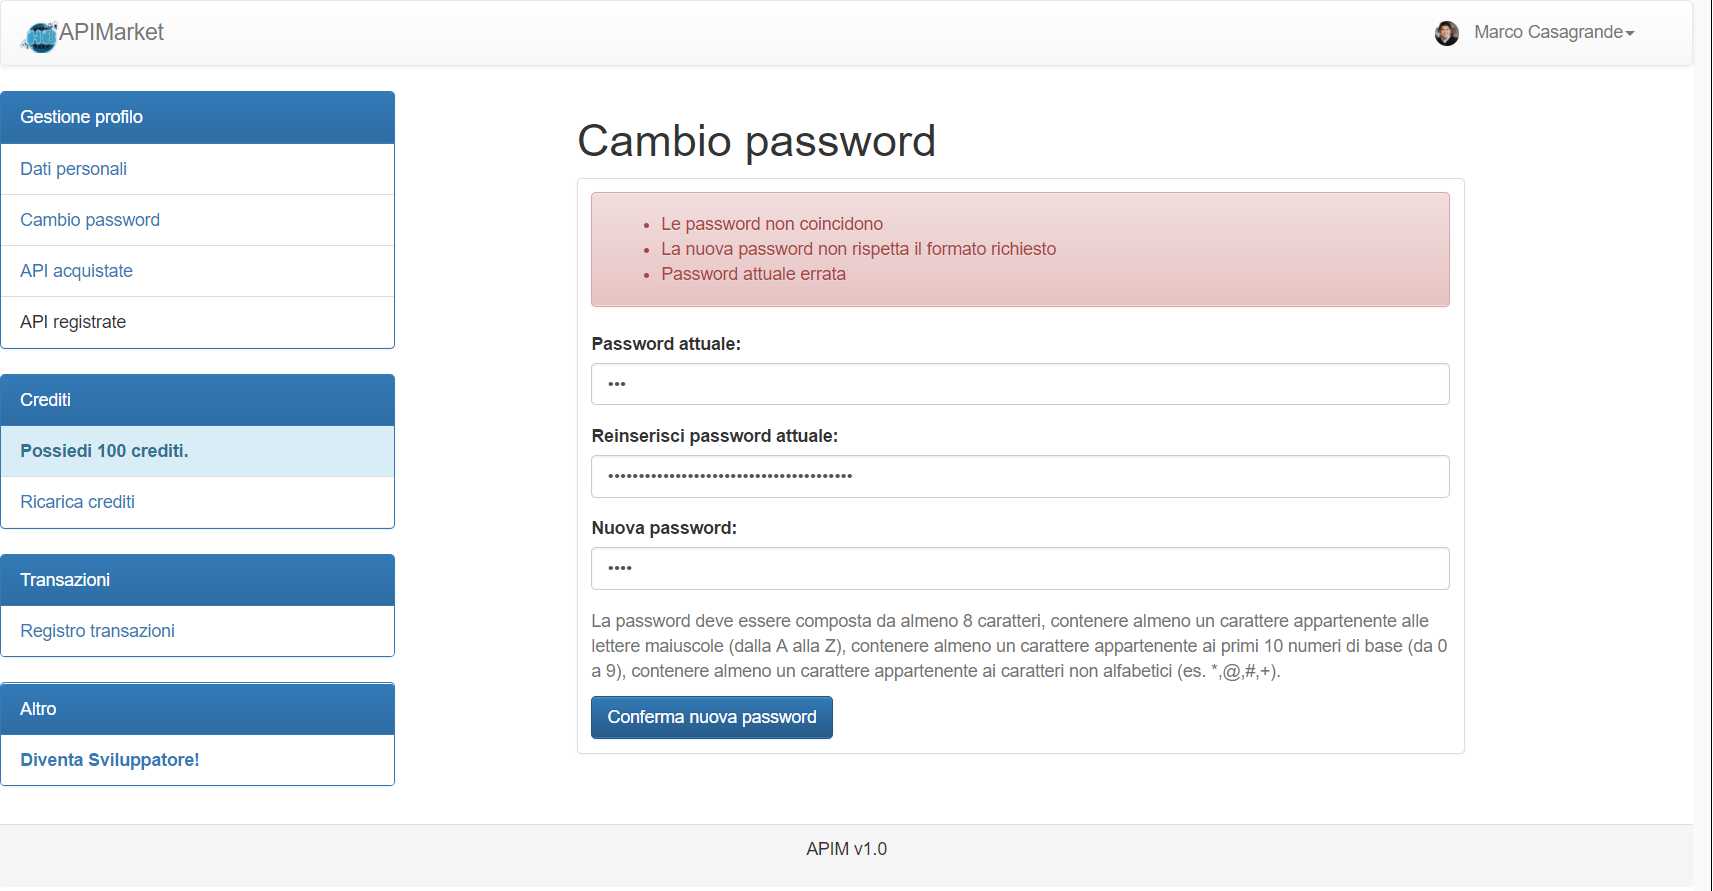
\includegraphics[scale=0.25]{img/APIM_ERRCambioPSW.png}}
	\caption{Errori cambio password}
\end{figure}

\subsection{Recupero password}
Se un utente dimentica la passowrd è possibile recuperarla. Se l'indirizzo email è correttamente registrato in \progetto, verrà inviata una email contenente la nuova password. Se l'email inserita non è corretta o registrata nell'API Market, visualizzerà un errore.
\label{Cambio password}
\begin{figure}[H]
	\centering
	\fbox{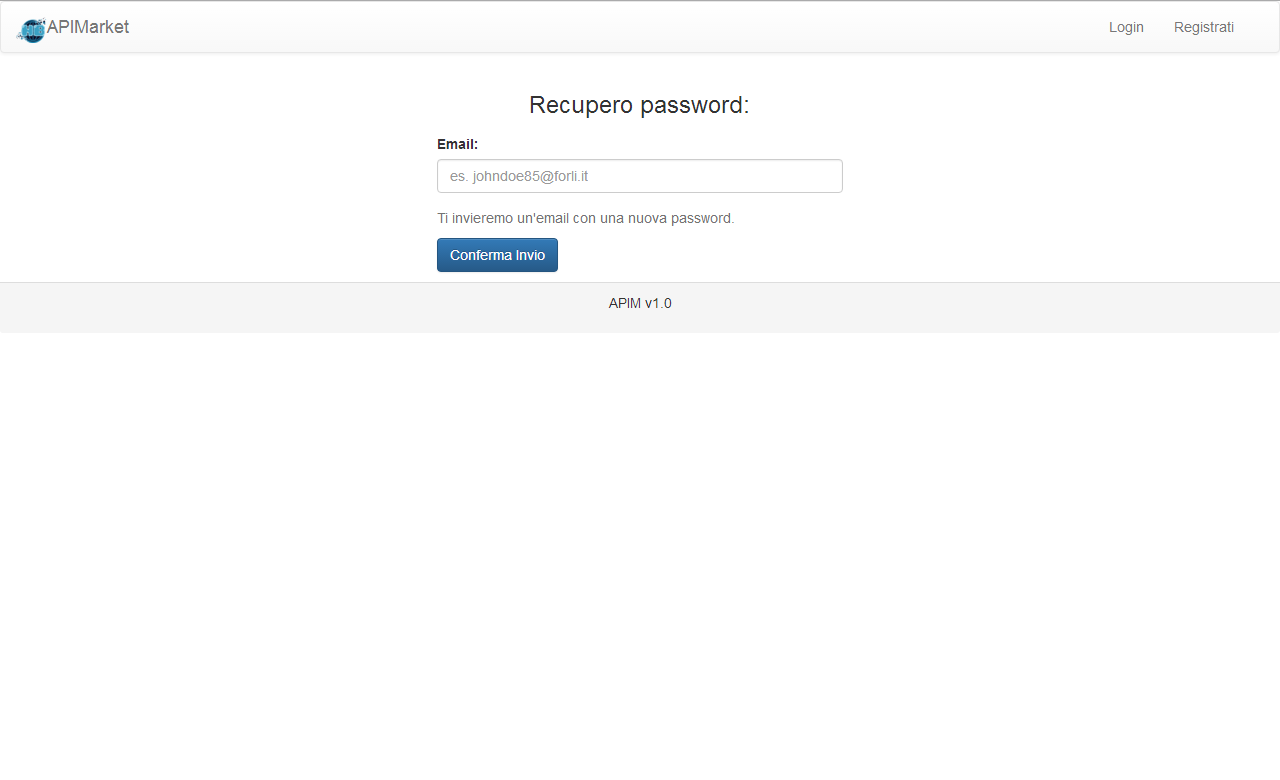
\includegraphics[scale=0.35]{img/APIM_recuperoPSW.png}}
	\caption{Cambio password}
\end{figure}
In caso di inserimento di una email valida, l'utente visualizzerà un messaggio di avvenuto invio della nuova password alla casella email inserita, come mostrato di seguito 

\label{Recupero password con successo}
\begin{figure}[H]
	\centering
	\fbox{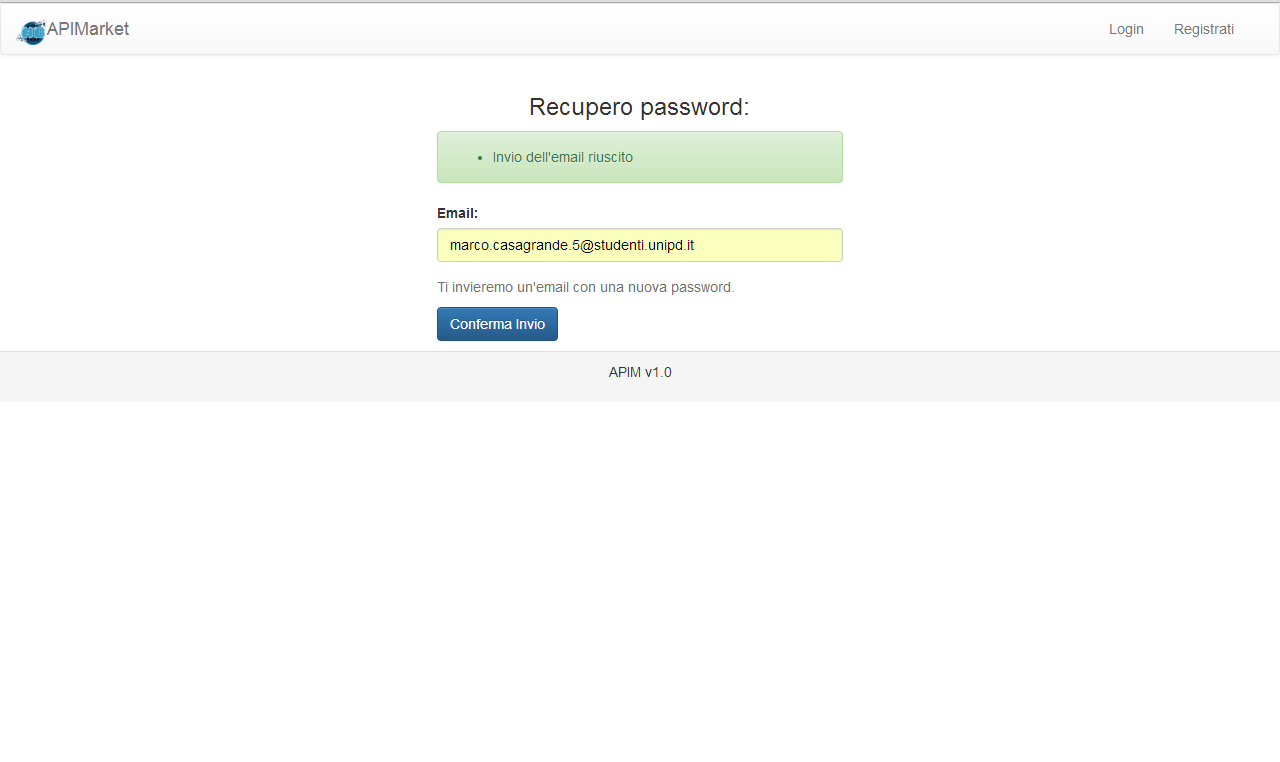
\includegraphics[scale=0.35]{img/APIM_recuperoOK.png}}
	\caption{Recupero password con successo}
\end{figure}

La nuova password arriverà via email, come mostrato di seguito.

\label{Nuova password}
\begin{figure}[H]
	\centering
	\fbox{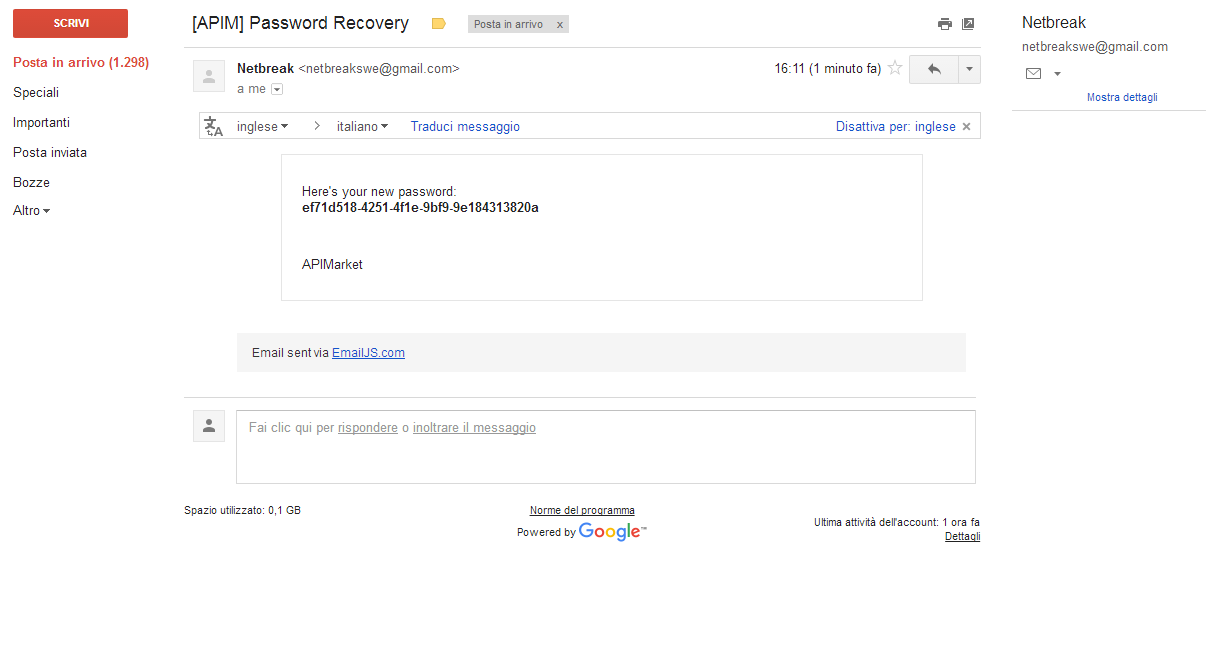
\includegraphics[scale=0.38]{img/APIM_nuovaPSW.png}}
	\caption{Nuova password}
\end{figure}



